\chapter{Introduction}\label{chap:intro}


Welcome to this \LaTeX{} thesis template. This template was originally created by the fabulous Dr Dom Brown, and updated by the amazing but not-quite-Dr Samuel Hunt. This template assumes you already know the basics of \LaTeX{}.


%Some examples of basic \LaTeX{} code are included throughout this chapter.

\section{Organisation}

The files needed for building this thesis are organised into several folders. In the root you will find uwethesis.tex, references.bib and count.sh. 

\begin{itemize}
\item \textit{uwethesis.tex} it the main tex file and links together the individual chapters which are intended to be written as separate .tex files. This is the file that you should run the various compile commands on.
\item \textit{references.bib} is where you should store your sources using a tool such as bibdesk to manage them. 
\item \textit{count.sh} is an optional utility tool for calculating the word count, you will need to update this as you add chapters. You can run this using \textbf{sh count.sh} from a terminal window. 
\end{itemize}



The 4 folders are organised as follows:

%Please use the relevant readme files in each folder, but in summary.

\begin{itemize}
\item Chapters: Contains the main .tex files, one for each chapter. You can also use sub-folders for grouping relevant chapters, i.e. background.
\item Setup: Contains various files for setting up the thesis, also includes .tex files for abstract, acknowledgements, etc.
\item Images: One of two places to store images (optional).
\item Papers: A good place to store your papers that need to be included (as PDFs).
\end{itemize}



\section{Images}

You may want to organise images in one of two ways. Either having one large folder of images, with sub-folders. Or having a image folder alongside each chapter. An example of both is given below:

\begin{figure}[h]
  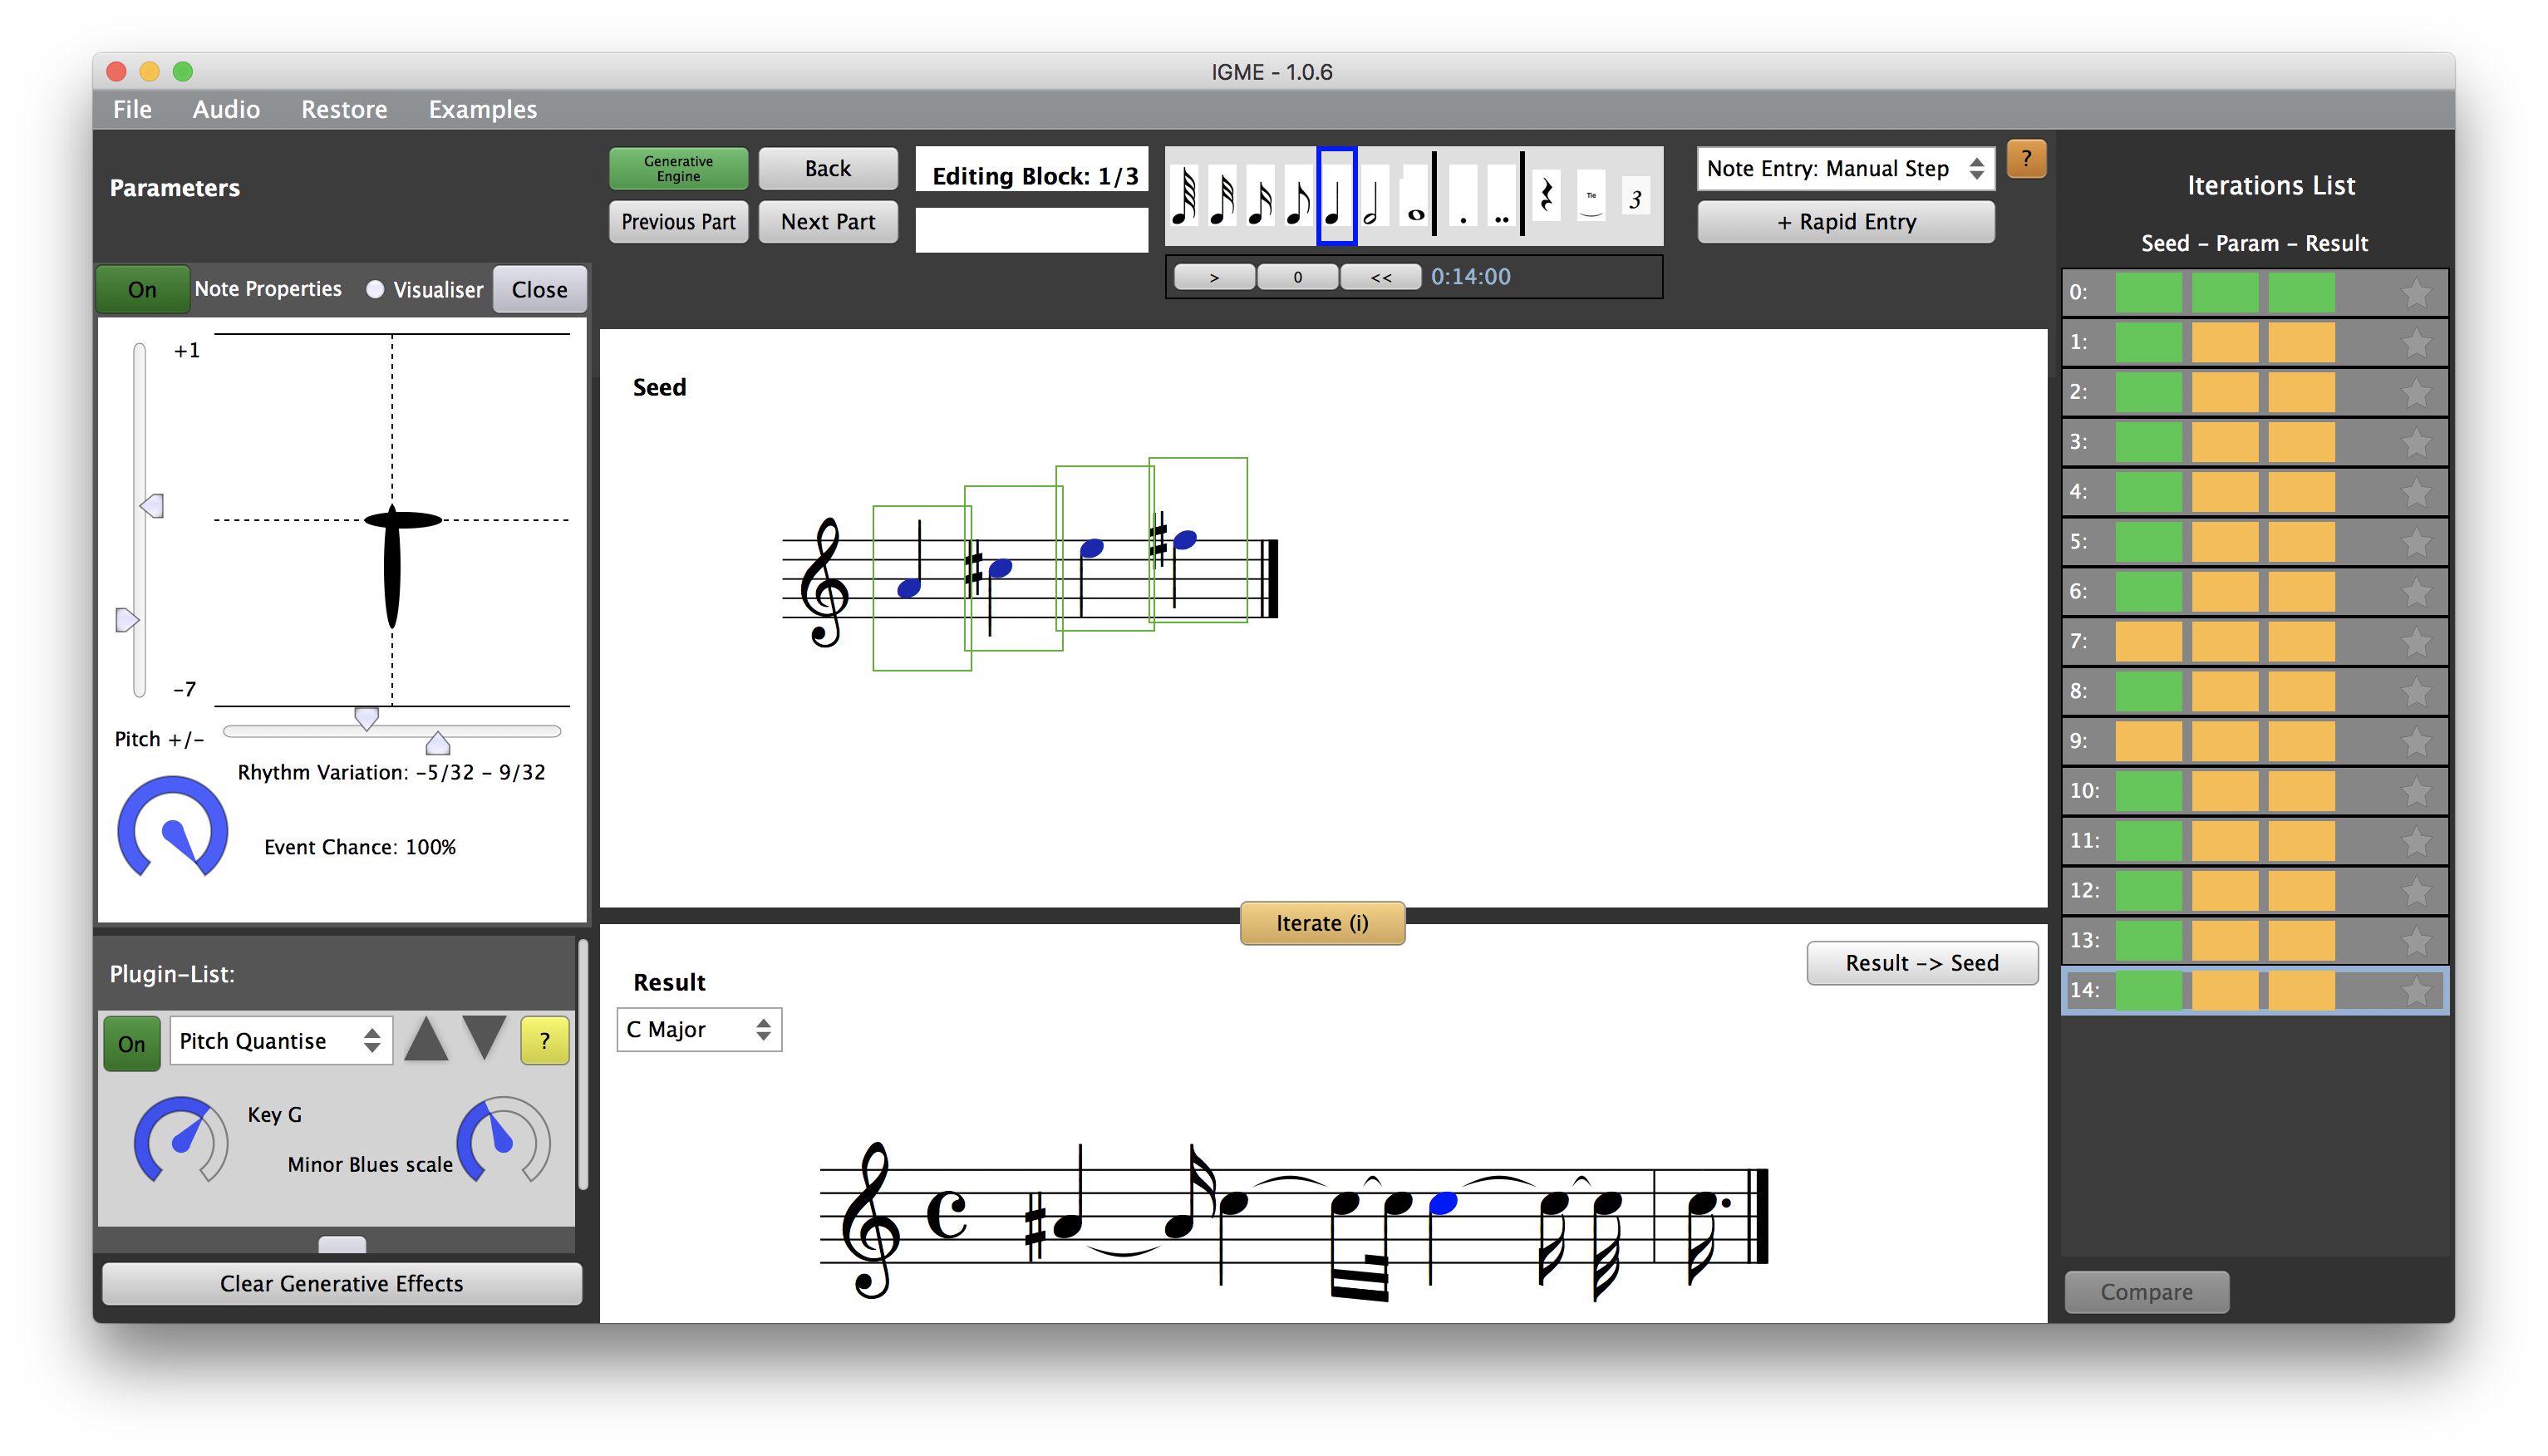
\includegraphics[width=\linewidth]{Images/EditView}
  \caption{Example of an image.}
  \label{fig:igme1}
\end{figure}

\begin{figure}[h]
\begin{center}
  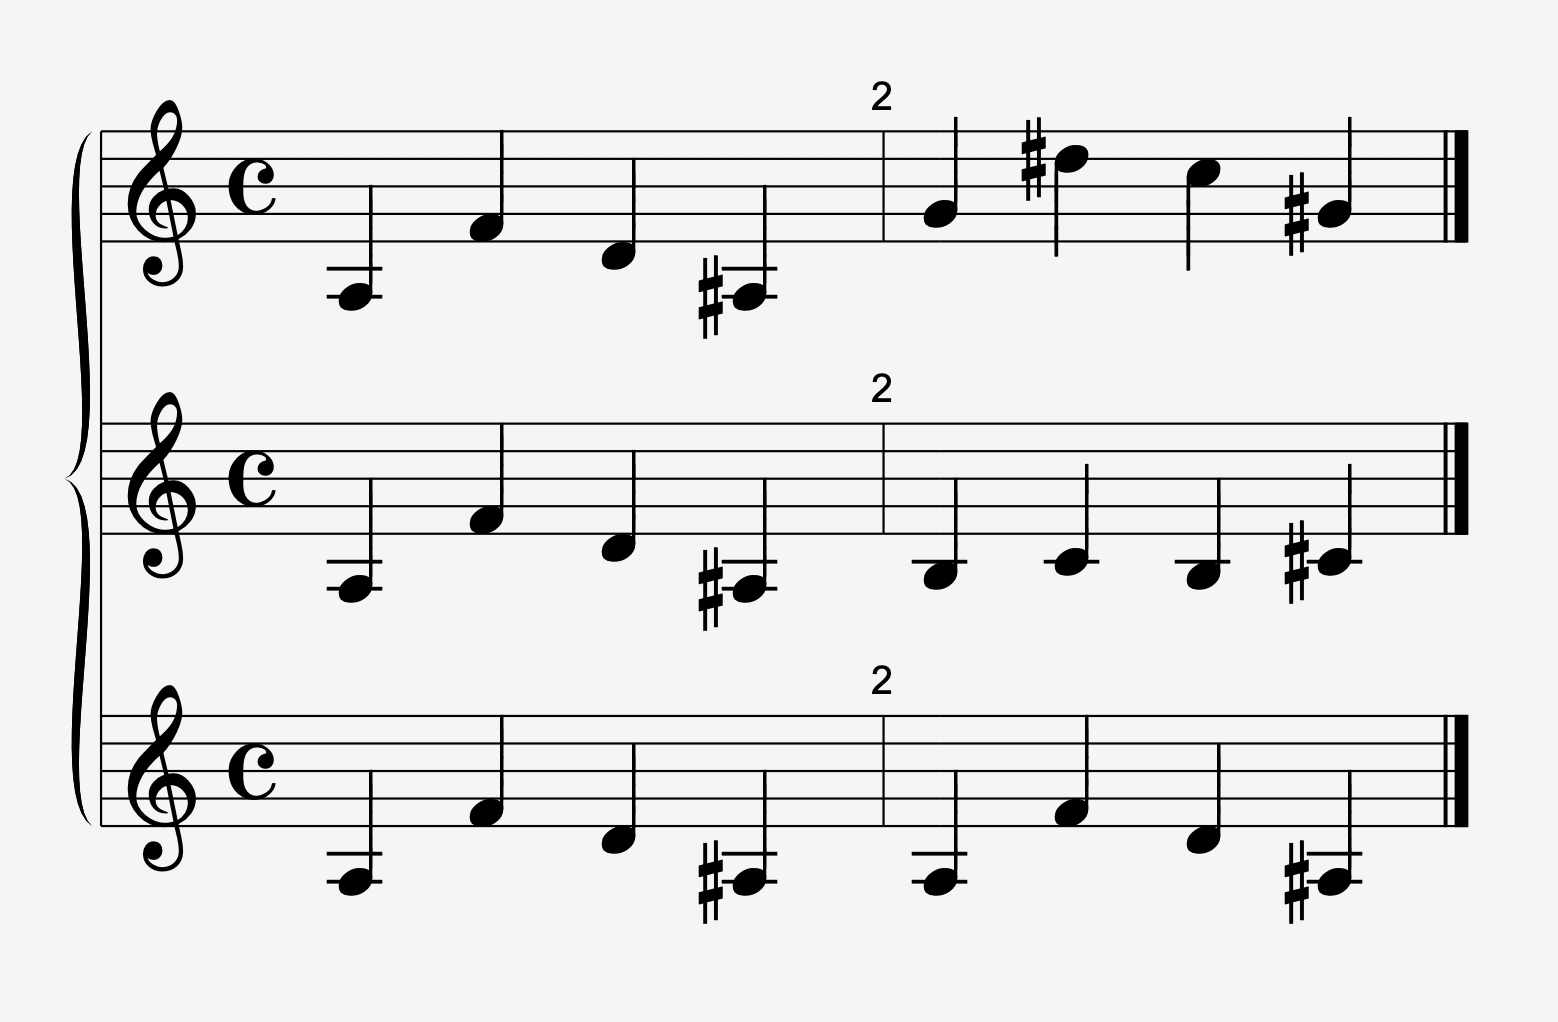
\includegraphics[width=0.6\linewidth]{Chapters/Evaluation/Images/partTypesScore}
  \caption{Another example of an image.}
  \label{fig:igme2}
  \end{center}
\end{figure}


\clearpage

\section{References and Citations}

\LaTeX{} will take care of building your reference list for you. Add your sources to the \textit{``references.bib''} file. Then you can cite using either \verb|\citet{} or \citep{}.| For example.

\begin{itemize}
\item \citet{hunt2020nime} studied interaction in computer-generated music systems - (uses \verb|\citet{}|).
\item IGME was built to study end-user computer-generated music \citep{hunt2020nime} - (uses \verb|\citep{}|).
\end{itemize}

References are automatically formatted as UWE Harvard. 

\subsection{Setup}

You will need to change your bib(la)tex command to use biber: ("biber" \%). This is what my Texmaker settings look like:

\begin{figure}[h]
  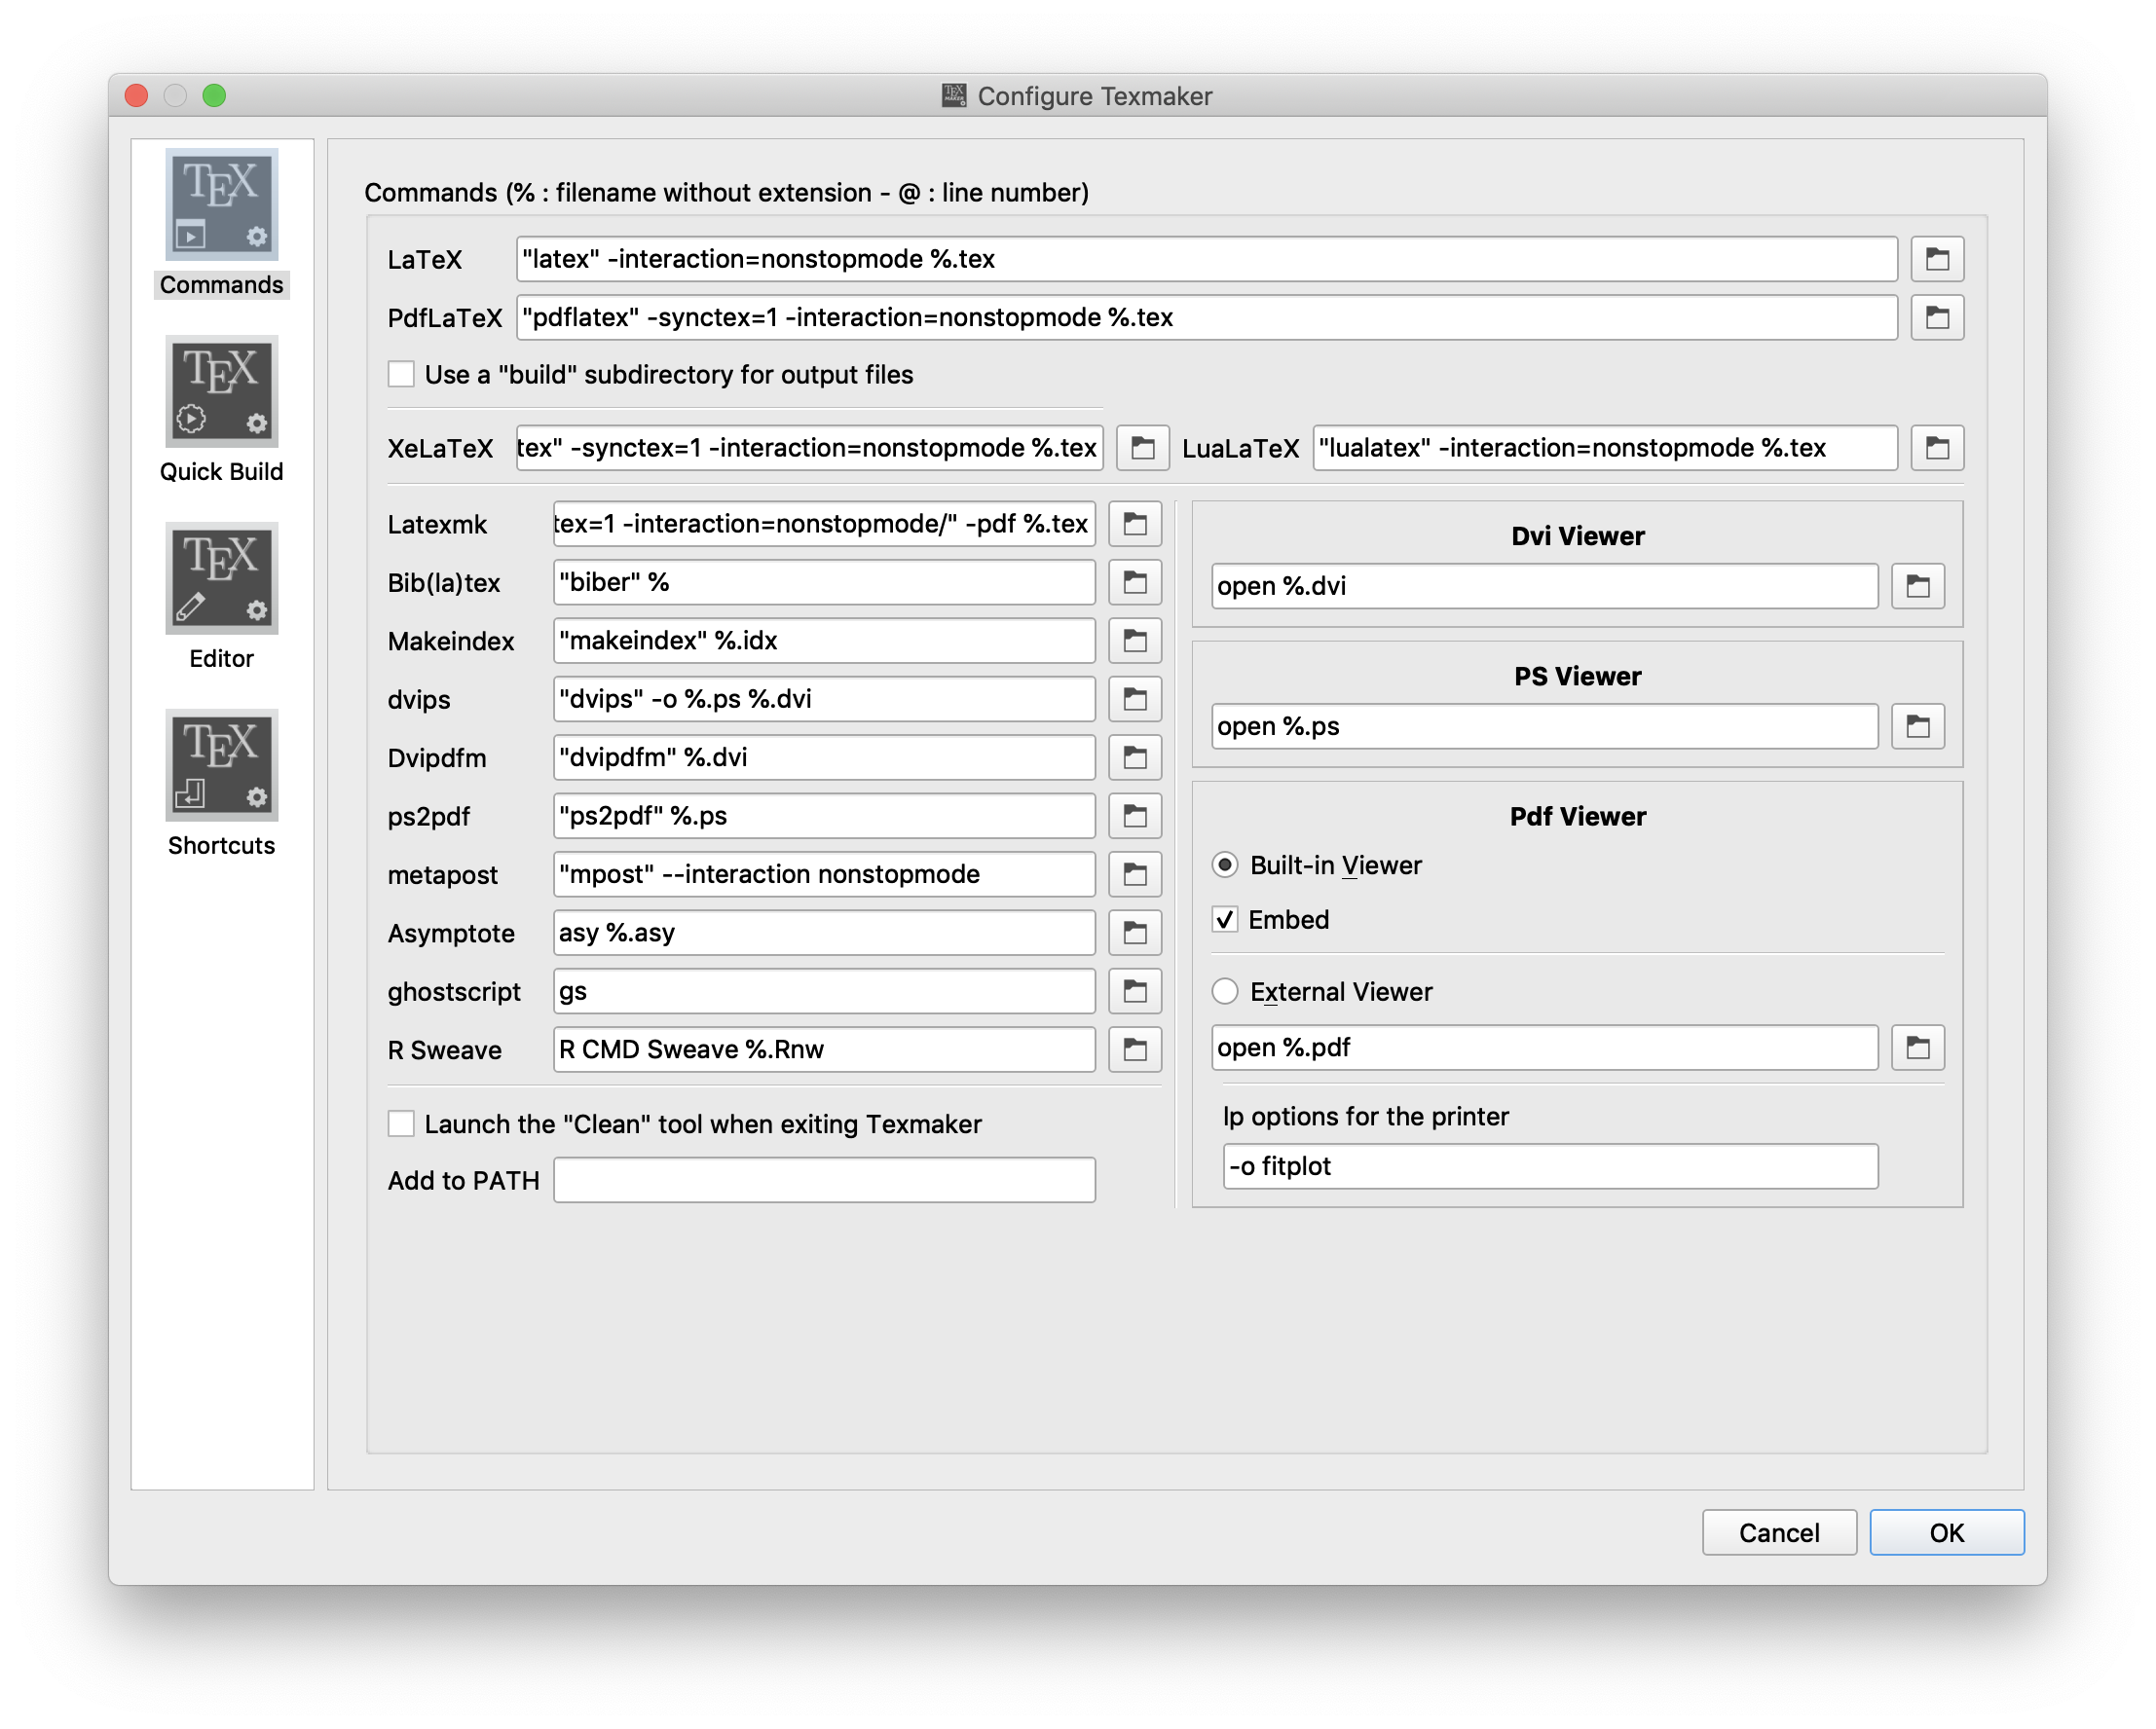
\includegraphics[width=\linewidth]{Images/texmaker}
  \caption{Settings in Texmaker.}
  \label{fig:igme1}
\end{figure}

\section{Building}

To build the thesis use:

\begin{enumerate}
\item XeLaTex
\item bibtex
\item XeLaTex
\item XeLaTex
\end{enumerate}

You can then just use \textit{XeLaTex} to rebuild the thesis, however references, figures numbers, and others wont get updated unless you do the full 4-step process.


 \section{Questions}
 
 Please email sjhunt93@gmail.com for any questions.


